\documentclass[10pt]{article}
\usepackage[USenglish]{babel}
\usepackage[useregional]{datetime2}
\usepackage{lipsum}
\usepackage{blindtext}
\usepackage{listings}
\usepackage[hashEnumerators,smartEllipses]{markdown}

\usepackage[most]{tcolorbox}
\definecolor{block-gray}{HTML}{ebedee}
\newtcolorbox{myquote}{colback=block-gray,grow to right by=-10mm,grow to left by=-10mm,
boxrule=0pt,boxsep=0pt,breakable}
\makeatletter
\def\quoteparse{\@ifnextchar`{\quotex}{\singlequote}}
\def\quotex#1{\@ifnextchar`{\triplequote\@gobble}{\doublequote}}
\makeatother
\def\singlequote#1`{[StartQ]#1[EndQ]\quoteON}
\def\doublequote#1``{[StartQQ]#1[EndQQ]\quoteON}
\long\def\triplequote#1```{\begin{myquote}\parskip 1ex#1\end{myquote}\quoteON}
\def\quoteON{\catcode``=\active}
\def\quoteOFF{\catcode``=12}
\quoteON
\def`{\quoteOFF \quoteparse}
\quoteOFF

\DTMlangsetup[en-US]{showdayofmonth=false}

\newcommand{\rfcId}{1.0}
\newcommand{\rfcTitle}{Service d'Annuaires Partagés}
\newcommand{\rfcAuthor}{Amine NAIM, Axel DELAS, Pierre BECKERS}
\newcommand{\rfcDate}{Decembre 2021}
\newcommand{\rfcInstitution}{Université Paul Sabatier}

% TABLE OF CONTENT
\usepackage{tocloft}
\renewcommand{\cftsecleader}{\cftdotfill{\cftdotsep}}
\renewcommand{\cftsubsecleader}{\cftdotfill{\cftdotsep}}
\renewcommand{\cftsubsubsecleader}{\cftdotfill{\cftdotsep}}
\renewcommand{\contentsname}{Table of Content}

% MARGINS
\usepackage{titlesec}
\titlelabel{\thetitle.\quad}
\usepackage{geometry} 
\geometry{
	a4paper,
	left=30mm,
	top=30mm,
	bottom=30mm,
	right=30mm
}
\setlength{\leftskip}{17pt}

% HEADER AND FOOTER
\usepackage{lastpage}
\usepackage{fancyhdr}
\pagestyle{fancyplain}
\fancyhead{}
\fancyfoot{}
\fancyhead[L]{RFC \rfcId}
\fancyhead[C]{\rfcTitle}
\fancyhead[R]{\rfcDate}
\fancyfoot[L]{\rfcAuthor} 
\fancyfoot[C]{} 
\fancyfoot[R]{[Page \thepage] \\} 
\renewcommand{\headrulewidth}{0pt} 
\renewcommand{\footrulewidth}{0pt} 
\setlength{\headheight}{13.6pt}

% FIGURE CAPTION SETUP
\usepackage{caption}
\captionsetup[figure]{font=small}


% FIRST PAGE
\usepackage{multicol}

% FONT
\usepackage{inconsolata}
\renewcommand{\familydefault}{\ttdefault}

%GLOSSARY : METTRE LES NOUVELLES ENTREES CI DESSOUS
\usepackage{glossaries}
\makeglossaries

\newglossaryentry{pdu}
{
    name=PDU,
    description={Unité de données du protocole (Protocol Data Unit)}
}

\newglossaryentry{charge utile}
{
    name=charge utile,
    description={Partie du paquet de données transmis qui contient l'information à transmettre. (en anglais \it payload)}
}

\newglossaryentry{requete}
{
    name=requête,
    description={Sollicitation d'un service par une entité pour faire une activité}
}

\newglossaryentry{reponse}
{
    name=réponse,
    description={Réponse à un évènement}
}


\begin{document}

\begin{multicols}{2}
	\begin{flushleft}
		Projet Semestre 5
	\end{flushleft}
\columnbreak
	\begin{flushright}
		\rfcAuthor \\
		\rfcInstitution
	\end{flushright}
\end{multicols}

\vspace{1in} { \center } \vspace{1in}

\begin{abstract}
	Le présent document explique le fonctionnement du service d'annuaires partagés. Il comporte cinq parties : une à propos des Unités de Données du Protocole (PDU) ; une au sujet de l'étape de connexion du client au serveur ; une concernant les échanges côté utilisateur ; une concernant les échanges côté administrateur et enfin un diagramme de séquence résumant les différents échanges possibles entre le client et le serveur. Chaque partie détaillera les types de requêtes et \gls{reponse}s communiquées entre le client et le serveur avec notamment des explications en mode DEBUG.
\end{abstract}
\pagebreak

\tableofcontents

\pagebreak

\section{Introduction}
{
    Le présent document détaille le fonctionnement d'un service d'annuaires partagés. Le service est basé sur une communication entre un client et un serveur. L'objectif de ce service est d'offir aux utilisateurs la possibilité de consulter et de maintenir un annuaire propre à chacun. Chaque contact comporte des informations telles que le nom, le prénom et l'adresse email des contacts ajoutés. D'autres telles que le numéro de téléphone ainsi que l'adresse postale restent des informations facultatives. Chaque utilisateur développe son annuaire en ajoutant ou en supprimant des contacts. Pour réguler les compte utilisateurs, un administrateur peut ajouter ou supprimer les utilisateurs et a tous les droits sur l'ensemble des annuaires.
}

\pagebreak

\section{Spécification des unités de données du protocole}
{
    
    Pour la réalisation de ce projet, les messages échangés entre le client et le serveur comporteront différents champs qui varient en nombre et en type selon le type de requête. Cette section décrit le format des unités de données du protocole (\gls{pdu}).
    \newline
    \begin{figure}[h]
        \centering
        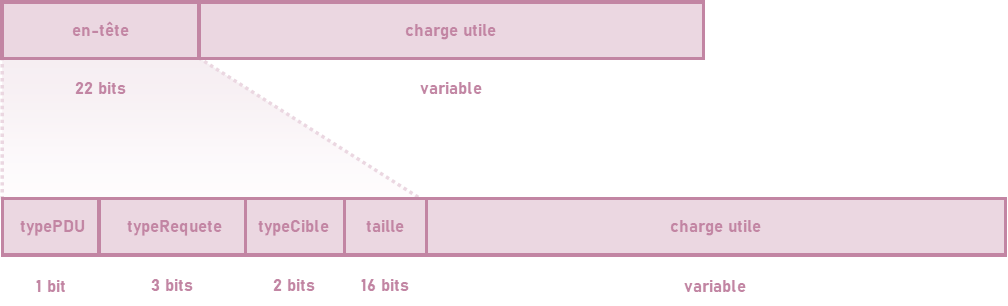
\includegraphics[width=\textwidth]{img/request.png}
        \caption{Format d'une unité de données du protocole de type \gls{requete}}
    \end{figure}
    \begin{figure}[h]
        \centering
        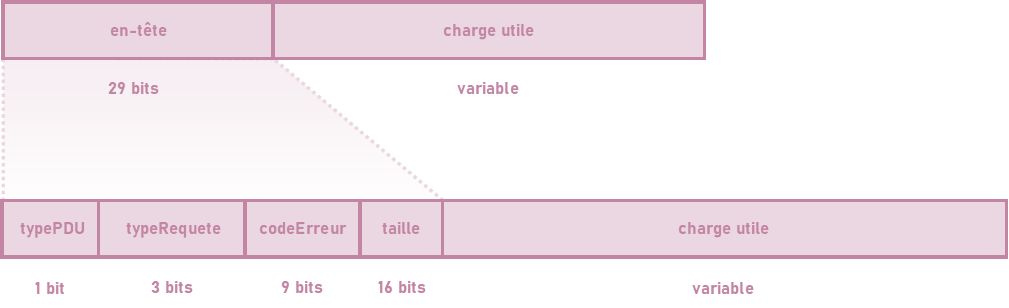
\includegraphics[width=\textwidth]{img/response.png}
        \caption{Format d'une unité de données du protocole de type \gls{reponse}}
    \end{figure}
    \subsection{Format de l'en-tête}
    {
        \subsubsection{typePDU}
        {
        1 bit. Il s'agit d'un champ de largeur fixe permettant d'indiquer le type de la PDU:\newline
        0 → Request ; 1 → Response.
        }
        \subsubsection{typeRequete}
        {
        3 bits. Il s'agit d'un champ de largeur fixe permettant d'indiquer le type de la requête.
        On en distingue 8, régissant les échanges entre le client et le serveur :
    	\begin{lstlisting}
            000 AUTH 
            001 ADD
            010 DELETE
            011 EDIT
            100 GET
            101 ALLOW
            110 SEARCH
            111 QUIT
        \end{lstlisting}
        }
        \subsubsection{typeCible}
        {
        2 bits. Champ spécifique à la requête. Il s'agit d'un champ de largeur fixe permettant d'indiquer le type de l'objet ciblé par la requête. Il en existe trois :
        \begin{lstlisting}
                    01 Utilisateur
                    10 Annuaire
                    11 Contact
        \end{lstlisting}
        On considère que si typeCible vaut 00, on omet sa valeur.
        }
        \subsubsection{taille}
        {
        16 bits. Champ commun aux deux types d'unités de données du protocole. Il s'agit d'un champ de largeur fixe permettant d'indiquer la longueur de la \gls{charge utile} (donnée) qui suit.
        }
        \subsubsection{codeErreur}
        {
        9 bits. Champ spécifique à la réponse. Chaque requête peut générer des codes d'erreurs tels que :\newline
    
        \indent\indent200 : Requete traitée avec succés.\newline
        \indent\indent400 : Identifiants incorrects.\newline
        \indent\indent401 : Erreur d'émission client.\newline
        \indent\indent402 : Requête au format incorrect.\newline
        \indent\indent403 : Erreur client inconnue.\newline
        \indent\indent501 : Erreur d'émission serveur.\newline
        \indent\indent502 : Erreur d'ouverture du fichier sur le serveur.\newline
        \indent\indent503 : Serveur injoignable.   
        }
    \subsection{Format de la \gls{charge utile}}
    {
        La \gls{charge utile} est un champ de taille nulle ou plus. Sa taille est indiquée par le champ 'taille' présent dans l'en-tête.
        \newline 
        \newline Il contient les informations associées à la requête/réponse. L'envoi de données est en termes de format de JSON.
    }
    }
    
}

\pagebreak

\section{Connexion}
{
    La connexion nécessite d'avoir un compte utilisateur créé au préalable par l'administrateur. Ceci étant fait, la connexion nécessite de passer par l'étape d'authentification sur le serveur avec un couple identifiant et mot de passe correct.
	\subsection{Exemple de requête côté interface utilisateur}
	{
	    \quoteON
	    ```
	    {
	       - Bienvenue sur votre service d'annuaires partagés -\newline
	       Identifiant : axdls31\newline
	       Mot de passe : ******\newline
	       Connexion effectuée avec succès.
	    }
	    ```
	    \quoteOFF
	}
	\subsection{Exemple de requête côté serveur en mode DEBUG}
	{
	    Pour la connexion, une requête de type AUTH, accompagnée du couple identifiant et mot de passe, est envoyée au serveur. Ce dernier renvoie une confirmation de succès ou d'échec : Code erreur 200 si le couple est correct, 400 sinon.
	    \quoteON
	    ```
	    {
	        DEBUG : [INFO] Connexion\newline
	        DEBUG : [REQUETE] AUTH axdls31 ******\newline
	        DEBUG : [CODE ERREUR] 200\newline
	        DEBUG : [AFFICHAGE] Connexion effectuée avec succès.
	    }
	    ```
	    \quoteOFF
	}
}

\pagebreak

\section{Description des échanges pour l'utilisateur}
{
    \subsection{Cas où l'utilisateur consulte son annuaire}
    {
        L'utilisateur doit pouvoir lire les données contenues dans son annuaire. Pour se faire, l'utilisateur doit sélectionner 'consulter mon annuaire' en indiquant le chiffre 1.
        \subsubsection{Exemple de requête côté interface utilisateur}
        {
        \quoteON
        ```
            \textbf{Amine - Utilisateur}\newline
            Sélectionner l'action souhaitée:\newline
            1 : Consulter l'annuaire\newline
            2 : Rechercher dans l'annuaire\newline
            3 : Consulter un annuaire distinct\newline
            4 : Ajouter un contact\newline
            5 : Modifier l'annuaire\newline
            6 : Supprimer un contact\newline
            7 : Consulter les utilisateurs autorisés à consulter mon annuaire\newline
            8 : Autoriser un utilisateur à consulter mon annuaire\newline
            9 : Déconnexion\newline
            Choix : 1\newline\newline
            Contenu de votre annuaire :\newline
            1) Admin Admin admin@stri.fr 8098350982 2 Chemin Upsitech 31000 TOULOUSE\newline
            2) Berners Tim tim.berners@email.com 0606060606 2 Rue de Upsitech 31000 TOULOUSE\newline
            3) Delas Axel axel.delas@stri.fr 0101010101 1 Palais de l'Elysée 75000 PARIS
        ```
        \quoteOFF
        }
        \subsubsection{Exemple de requête côté serveur en mode DEBUG}
        {
            Consulter son annuaire est effectué en envoyant une requête de type GET au serveur.
        \quoteON
        ```
            DEBUG : [INFO] Consultation de l'annuaire\newline
            DEBUG : [INFO] Lecture de l'annuaire du user courant\newline
            DEBUG : [REQUETE] GET amine.naim@stri.fr\newline
            DEBUG : [INFO] Affichage des contacts lus\newline
            DEBUG : [CODE ERREUR] 200\newline
            DEBUG : [AFFICHAGE] Admin Admin admin@stri.fr 8098350982 2 Chemin Upsitech 31000 TOULOUSE\newline
            DEBUG : [AFFICHAGE] Berners Tim tim.berners@email.com 0606060606 2 Rue de Upsitech 31000 TOULOUSE\newline
            DEBUG : [AFFICHAGE] Delas Axel axel.delas@stri.fr 0101010101 1 Palais de l'Elysée 75000 PARIS
        ```
        \quoteOFF
        }
    }
    \subsection{Cas où l'utilisateur recherche dans l'annuaire}
    {
        L'utilisateur doit pouvoir effectuer une recherche parmi les données présentes dans son annuaire, l'objectif étant de lire spécifiquement un contact. Ceci peut être fait en saisissant le chiffre 2 et ainsi choisir 'Rechercher dans l'annuaire' figurant dans le menu.
        \subsubsection{Exemple de requête côté interface utilisateur}
        {
        \quoteON
        ```
            \textbf{Amine - Utilisateur}\newline
            Sélectionner l'action souhaitée:\newline
            1 : Consulter l'annuaire\newline
            2 : Rechercher dans l'annuaire\newline
            3 : Consulter un annuaire distinct\newline
            4 : Ajouter un contact\newline
            5 : Modifier l'annuaire\newline
            6 : Supprimer un contact\newline
            7 : Consulter les utilisateurs autorisés à consulter mon annuaire\newline
            8 : Autoriser un utilisateur à consulter mon annuaire\newline
            9 : Déconnexion\newline
            Choix : 2\newline\newline
            Email du contact : axel.delas@stri.fr\newline\newline
            Informations de axel.delas@stri.fr :\newline
            Delas Axel axel.delas@stri.fr 0101010101 1 Palais de l'Elysée 75000 PARIS
        ```
        \quoteOFF
        }
        \subsubsection{Exemple de requête côté serveur en mode DEBUG}
        {
            Rechercher dans l'annuaire un contact spécifique est effectué d'une part grâce à la requête de type GET mais d'une autre part grâce à la requête de type SEARCH. 
        \quoteON
        ```
            DEBUG : [INFO] Consultation de l'annuaire\newline
            DEBUG : [INFO] Lecture de l'annuaire du user courant\newline
            DEBUG : [REQUETE] GET amine.naim@stri.fr\newline
            DEBUG : [INFO] Recherche du contact axel.delas@stri.fr\newline
            DEBUG : [REQUETE] SEARCH axel.delas@stri.fr\newline
            DEBUG : [INFO] Lecture du contact axel.delas@stri.fr\newline
            DEBUG : [REQUETE] GET axel.delas@stri.fr\newline
            DEBUG : [INFO] Affichage des contacts de axel.delas@stri.fr\newline
            DEBUG : [CODE ERREUR] 200\newline
            DEBUG : [AFFICHAGE] Delas Axel axel.delas@stri.fr 0101010101 1 Palais de l'Elysée 75000 PARIS
        ```
        \quoteOFF
        }
    }
    \subsection{Cas où l'utilisateur consulte un annuaire distinct}
    {
        L'utilisateur doit pouvoir consulter un annuaire distinct appartenant à un utilisateur qui a donné l'autorisation au préalable. Ainsi, l'utilisateur saisie le chiffre 3 afin de choisir 'Consulter un annuaire distinct' figurant dans le menu.
        \subsubsection{Exemple de requête côté interface utilisateur}
        {
            \label{Consulter annuaire distinct user}
        \quoteON
        ```
            \textbf{Axel - Utilisateur}\newline
            Sélectionner l'action souhaitée:\newline
            1 : Consulter l'annuaire\newline
            2 : Rechercher dans l'annuaire\newline
            3 : Consulter un annuaire distinct\newline
            4 : Ajouter un contact\newline
            5 : Modifier l'annuaire\newline
            6 : Supprimer un contact\newline
            7 : Consulter les utilisateurs autorisés à consulter mon annuaire\newline
            8 : Autoriser un utilisateur à consulter mon annuaire\newline
            9 : Déconnexion\newline
            Choix : 3\newline\newline
            Email de l'utilisateur : amine.naim@stri.fr\newline\newline
            Contenu de l'annuaire de Amine Naim :\newline
            1) Admin Admin admin@stri.fr 8098350982 2 Chemin Upsitech 31000 TOULOUSE\newline
            2) Axel Delas axel.delas@stri.fr 0101010101 1 Palais de l'Elysée 75000 PARIS\newline
            3) Pierre Beckers pierre.beckers@stri.fr 9275028408 20 Rue du Chêne 31000 TOULOUSE
        ```
        \quoteOFF
        }
        \subsubsection{Exemple de requête côté serveur en mode DEBUG}
        {
            \label{Consulter annuaire distinct serveur}
            Lire un annuaire distinct est effectué en envoyant une requête de type GET.
        \quoteON
        ```
            DEBUG : [INFO] Consultation d'un annuaire distinct\newline
            DEBUG : [INFO] Lecture de l'annuaire du user courant\newline
            DEBUG : [REQUETE] GET axel.delas@stri.fr\newline
            DEBUG : [INFO] Lecture de l'annuaire de amine.naim@stri.fr\newline
            DEBUG : [REQUETE] GET amine.naim@stri.fr\newline
            DEBUG : [INFO] Affichage des contacts de amine.naim@stri.fr\newline
            DEBUG : [CODE ERREUR] 200\newline
            DEBUG : [AFFICHAGE] Admin Admin admin@stri.fr 8098350982 2 Chemin Upsitech 31000 TOULOUSE\newline
            DEBUG : [AFFICHAGE] Axel Delas axel.delas@stri.fr 0101010101 1 Palais de l'Elysée 75000 PARIS\newline
            DEBUG : [AFFICHAGE] Pierre Beckers pierre.beckers@stri.fr 9275028408 20 Rue du Chêne 31000 TOULOUSE
        ```
        \quoteOFF
        }
    }
    \subsection{Cas où l'utilisateur ajoute un contact}
    {
        Ici l'utilisateur doit pouvoir ajouter un nouveau contact dans son annuaire en renseignant les informations obligatoires telles que le nom, le prénom et l'adresse email ou encore le numéro de téléphone et l'adresse postale qui sont tous deux facultatifs. Pour se faire, l'utilisateur doit sélectionner 'Ajouter un contact' en saisissant le chiffre 4.
        \subsubsection{Exemple de requête côté interface utilisateur}
        {
        \quoteON
        ```
            \textbf{Amine - Utilisateur}\newline
            Sélectionner l'action souhaitée:\newline
            1 : Consulter l'annuaire\newline
            2 : Rechercher dans l'annuaire\newline
            3 : Consulter un annuaire distinct\newline
            4 : Ajouter un contact\newline
            5 : Modifier l'annuaire\newline
            6 : Supprimer un contact\newline
            7 : Consulter les utilisateurs autorisés à consulter mon annuaire\newline
            8 : Autoriser un utilisateur à consulter mon annuaire\newline
            9 : Déconnexion\newline
            Choix : 4\newline\newline
            Email du nouveau contact : axel.delas@stri.fr\newline
            Nouveau contact ajouté avec succès.
        ```
        \quoteOFF
        }
        \subsubsection{Exemple de requête côté serveur en mode DEBUG}
        {
            Ajouter un nouveau contact dans l'annuaire envoie une requête de type ADD au serveur.
        \quoteON
        ```
            DEBUG : [INFO] Ajout d'un nouveau contact\newline
            DEBUG : [INFO] Ajout du contact axel.delas@stri.fr\newline
            DEBUG : [REQUETE] ADD axel.delas@stri.fr\newline
            DEBUG : [CODE ERREUR] 200\newline
            DEBUG : [AFFICHAGE] Nouveau contact ajouté avec succès.
        ```
        \quoteOFF
        }
    }
    \subsection{Cas où l'utilisateur modifie l'annuaire}
    {
        Ici l'utilisateur doit pouvoir modifier une information appartenant à l'un des contacts faisant parti de l'annuaire. L'utilisateur doit choisir 'Modifier l'annuaire' en saisissant le chiffre 5.
        \subsubsection{Exemple de requête côté interface utilisateur}
        {
            \label{Modifier l'annuaire côté user}
        \quoteON
        ```
            \textbf{Axel - Utilisateur}\newline
            Sélectionner l'action souhaitée:\newline
            1 : Consulter l'annuaire\newline
            2 : Rechercher dans l'annuaire\newline
            3 : Consulter un annuaire distinct\newline
            4 : Ajouter un contact\newline
            5 : Modifier l'annuaire\newline
            6 : Supprimer un contact\newline
            7 : Consulter les utilisateurs autorisés à consulter mon annuaire\newline
            8 : Autoriser un utilisateur à consulter mon annuaire\newline
            9 : Déconnexion\newline
            Choix : 5\newline\newline
            Contenu de votre annuaire :\newline
            1) Admin Admin admin@stri.fr\newline
            2) Berners Tim tim.berners@email.com\newline
            3) Naim Amine amine.naim@abcd.net\newline\newline
            Email du contact à modifier : tim.berners@email.com\newline\newline
            Information à modifier : email\newline
            Nouvelle information : tim.berners@stri.fr\newline
            Contact modifié avec succès.
        ```
        \quoteOFF
        }
        \subsubsection{Exemple de requête côté serveur en mode DEBUG}
        {
            \label{Modifier un user côté serveur}
            La modification une information associée à un contact effectue plusieurs types de requêtes dont une requête de type GET et une requête de type EDIT.
        \quoteON
        ```
            DEBUG : [INFO] Modification d'un contact\newline
            DEBUG : [INFO] Lecture de l'annuaire du user courant\newline
            DEBUG : [REQUETE] GET axel.delas@stri.fr\newline
            DEBUG : [AFFICHAGE] Admin Admin admin@stri.fr\newline
            DEBUG : [AFFICHAGE] Berners Tim tim.berners@email.com\newline
            DEBUG : [AFFICHAGE] Naim Amine amine.naim@abcd.net\newline
            DEBUG : [INFO] Lecture du contact tim.berners@email.com\newline
            DEBUG : [INFO] Modification du contact tim.berners@email.com\newline
            DEBUG : [REQUETE] EDIT tim.berners@email.com tim.berners@stri.fr\newline
            DEBUG : [CODE ERREUR] 200\newline
            DEBUG : [AFFICHAGe] Contact modifié avec succès.
        ```
        \quoteOFF
        }
    }
    \subsection{Cas où l'utilisateur supprime un contact}
    {
        L'utilisateur doit pouvoir supprimer un contact de son annuaire. Ce dernier doit choisir 'Supprimer un contact' figurant dans le menu en saisissant le chiffre 6.
        \subsubsection{Exemple de requête côté interface utilisateur}
        {
        \quoteON
        ```
            \textbf{Amine - Utilisateur}\newline
            Sélectionner l'action souhaitée:\newline
            1 : Consulter l'annuaire\newline
            2 : Rechercher dans l'annuaire\newline
            3 : Consulter un annuaire distinct\newline
            4 : Ajouter un contact\newline
            5 : Modifier l'annuaire\newline
            6 : Supprimer un contact\newline
            7 : Consulter les utilisateurs autorisés à consulter mon annuaire\newline
            8 : Autoriser un utilisateur à consulter mon annuaire\newline
            9 : Déconnexion\newline
            Choix : 6\newline\newline
            Contenu de votre annuaire :\newline
            1) Admin Admin admin@stri.fr 8098350982 2 Chemin Upsitech 31000 TOULOUSE\newline
            2) Berners Tim tim.berners@email.com 0606060606 2 Rue de Upsitech 31000 TOULOUSE\newline
            3) Axel Delas axel.delas@stri.fr 0101010101 1 Palais de l'Elysée 75000 PARIS\newline\newline
            Email du contact à supprimer : axel.delas@stri.fr\newline
            Contact supprimé avec succès.
        ```
        \quoteOFF
        }
        \subsubsection{Exemple de requête côté serveur en mode DEBUG}
        {
            Supprimer un contact de l'annuaire nécessite d'utiliser plusieurs types de requêtes tels que GET et DELETE.
        \quoteON
        ```
            DEBUG : [INFO] Suppression d'un contact\newline
            DEBUG : [INFO] Lecture de l'annuaire du user courant\newline
            DEBUG : [REQUETE] GET amine.naim@stri.fr\newline
            DEBUG : [AFFICHAGE] Admin Admin admin@stri.fr 8098350982 2 Chemin Upsitech 31000 TOULOUSE\newline
            DEBUG : [AFFICHAGE] Berners Tim tim.berners@email.com 0606060606 2 Rue de Upsitech 31000 TOULOUSE\newline
            DEBUG : [AFFICHAGE] Axel Delas axel.delas@stri.fr 0101010101 1 Palais de l'Elysée 75000 PARIS\newline
            DEBUG : [INFO] Suppression du contact axel.delas@stri.fr\newline
            DEBUG : [REQUETE] DELETE axel.delas@stri.fr\newline
            DEBUG : [CODE ERREUR] 200\newline
            DEBUG : [AFFICHAGE] Contact supprimé avec succès.
        ```
        \quoteOFF
        }
    }
    \subsection{Cas où l'utilisateur affiche les contacts autorisés à consulter son annuaire}
    {
        L'utilisateur doit pouvoir afficher les contacts qu'il a au préalable autorisé à consulter son annuaire. Pour se faire, l'utilisateur choisi 'Consulter les utilisateurs autorisés à consulter mon annuaire' en saisissant le chiffre 7.
        \subsubsection{Exemple de requête côté interface utilisateur}
        {
        \quoteON
        ```
            \textbf{Axel - Utilisateur}\newline
            Sélectionner l'action souhaitée:\newline
            1 : Consulter l'annuaire\newline
            2 : Rechercher dans l'annuaire\newline
            3 : Consulter un annuaire distinct\newline
            4 : Ajouter un contact\newline
            5 : Modifier l'annuaire\newline
            6 : Supprimer un contact\newline
            7 : Consulter les utilisateurs autorisés à consulter mon annuaire\newline
            8 : Autoriser un utilisateur à consulter mon annuaire\newline
            9 : Déconnexion\newline
            Choix : 7\newline\newline
            1) tim.berners@email.com
        ```
        \quoteOFF
        }
        \subsubsection{Exemple de requête côté serveur en mode DEBUG}
        {
            L'affichage des utilisateurs autorisés à consulter l'annuaire est effectuée à travers une requête de type GET au serveur.
        \quoteON
        ```
            DEBUG : [INFO] Affichage des users autorisés à consulter l'annuaire\newline
            DEBUG : [INFO] Lecture de l'annuaire du user courant\newline
            DEBUG : [REQUETE] GET axel.delas@stri.fr\newline
            DEBUG : [INFO] Lecture des contacts ayant l'autorisation\newline
            DEBUG : [REQUETE] WHO\_ALLOW axel.delas@stri.fr\newline
            DEBUG : [CODE ERREUR] 200\newline
            DEBUG : [AFFICHAGE] tim.berners@email.com
        ```
        \quoteOFF
        }
    }
    \subsection{Cas où l'utilisateur autorise à consulter son annuaire}
    {
        L'utilisateur doit pouvoir autoriser un utiliseur distinct à consulter son annuaire. Pour se faire, l'utilisateur choisi 'Autoriser un utilisateur à consulter mon annuaire' figurant dans le menu en saisissant le chiffre 8.
        \subsubsection{Exemple de requête côté interface utilisateur}
        {
        \quoteON
        ```
            \textbf{Axel - Utilisateur}\newline
            Sélectionner l'action souhaitée:\newline
            1 : Consulter l'annuaire\newline
            2 : Rechercher dans l'annuaire\newline
            3 : Consulter un annuaire distinct\newline
            4 : Ajouter un contact\newline
            5 : Modifier l'annuaire\newline
            6 : Supprimer un contact\newline
            7 : Consulter les utilisateurs autorisés à consulter mon annuaire\newline
            8 : Autoriser un utilisateur à consulter mon annuaire\newline
            9 : Déconnexion\newline
            Choix : 8\newline\newline
            Adresse email de l'utilisateur à autoriser : amine.naim@stri.fr\newline
            Autorisation ajoutée avec succès.
        ```
        \quoteOFF
        }
        \subsubsection{Exemple de requête côté serveur en mode DEBUG}
        {
            Autoriser un utilisateur à consulter son annuaire effectue d'une part une requête de type GET et d'une autre part une requête ALLOW.
        \quoteON
        ```
            DEBUG : [INFO] Autorisation d'un user à consulter l'annuaire\newline
            DEBUG : [INFO] Lecture de l'annuaire du user courant\newline
            DEBUG : [REQUETE] GET axel.delas@stri.fr\newline
            DEBUG : [INFO] Ajout de l'autorisation à amine.naim@stri.fr\newline
            DEBUG : [REQUETE] ALLOW amine.naim@stri.fr\newline
            DEBUG : [CODE ERREUR] 200\newline
            DEBUG : [AFFICHAGE] Autorisation ajoutée avec succès.
        ```
        \quoteOFF
        }
    }

    \subsection{Cas où l'utilisateur se déconnecte}
    {
        L'utilisateur doit pouvoir se déconnecter du serveur de l'application qui permet de mettre fin à la connexion entre le client et le serveur. Pour se faire, l'utilisateur doit saisir le chiffre 10 et ainsi choisir 'Déconnexion' dans le menu.
    	\subsubsection{Exemple de requête côté interface utilisateur}
    	{
    	    \label{Déconnexion côté user}
        \quoteON
        ```
            \textbf{Axel - Utilisateur}\newline
            Sélectionner l'action souhaitée:\newline
            1 : Consulter l'annuaire\newline
            2 : Rechercher dans l'annuaire\newline
            3 : Consulter un annuaire distinct\newline
            4 : Ajouter un contact\newline
            5 : Modifier l'annuaire\newline
            6 : Supprimer un contact\newline
            7 : Consulter les utilisateurs autorisés à consulter mon annuaire\newline
            8 : Autoriser un utilisateur à consulter mon annuaire\newline
            9 : Déconnexion\newline
            Choix : 9\newline\newline
            Déconnexion effectuée avec succès.
        ```
        \quoteOFF
        }
    	\subsubsection{Exemple de requête côté serveur en mode DEBUG}
    	{
    	    \label{Déconnexion côté serveur}
    	    La déconnexion se fait grâce à l'envoie d'une requête de type QUIT au serveur.
	    \quoteON
	    ```
	        DEBUG : [INFO] Déconnexion\newline
	        DEBUG : [INFO] Déconnexion du user courant\newline
	        DEBUG : [REQUETE] QUIT axel.delas@stri.fr\newline
	        DEBUG : [CODE ERREUR] 200\newline
	        DEBUG : [AFFICHAGE] Déconnexion effectuée avec succès.
	    ```
	    \quoteOFF
    	}
    }
}

\pagebreak

\section{Description des échanges pour l'administrateur}
{
    \subsection{Cas où l'administrateur ajoute un utilisateur}
    {
        L'administrateur doit pouvoir ajouter un nouvel utilisateur au sein du service d'annuaires partagés. A l'ajout de ce dernier, un annuaire lui ait créé et associé. Pour se faire, l'administrateur doit saisir le chiffre 1 et ainsi choisir 'Ajouter un utilisateur' figurant dans le menu
        \subsubsection{Exemple de requête côté interface utilisateur}
        {
        \quoteON
        ```
            \textbf{Axel - Administrateur}\newline
            Sélectionner l'action souhaitée:\newline
            1 : Ajouter un utilisateur\newline
            2 : Supprimer un utilisateur\newline
            3 : Modifier un utilisateur\newline
            4 : Consulter un annuaire distinct\newline
            5 : Afficher les utilisateurs de l'application\newline
            6 : Déconnexion\newline
            Choix : 1\newline\newline
            Informations du nouvel utilisateur :\newline
            Nom : Delas\newline
            Prénom : Axel\newline
            Email : axel.delas@stri.fr\newline
            Numéro de tel : 0101010101\newline
            Adresse postale : 1 Palais de l'Elysée 75000 PARIS \newline
            Nouvel utilisateur crée avec succès.
        ```
        \quoteOFF
        }
        \subsubsection{Exemple de requête côté serveur en mode DEBUG}
        {
            Ajouter un nouvel utilisateur dans le service est effectué en envoyant une requête de type ADD au serveur.
            \quoteON
            ```
                DEBUG : [INFO] Ajout d'un nouveau user\newline
                DEBUG : [INFO] Ajout de axel.delas@stri.fr\newline
                DEBUG : [REQUETE] ADD Delas Axel axel.delas@stri.fr 0101010101 1 Rue de l'Elysée 75000 PARIS\newline
                DEBUG : [CODE ERREUR] 200\newline
                DEBUG : [AFFICHAGE] Nouvel utilisateur crée avec succès
            ```
            \quoteOFF
        }
    }
    \subsection{Cas où l'administrateur supprime un utilisateur}
    {
        L'administrateur doit pouvoir supprimer un utilisateur au sein du service d'annuaires partagés. De plus, en supprimant le compte de ce dernier, son annuaire partagé est également supprimé. Pour se faire, l'administrateur doit saisir le chiffre 2 afin de choisir 'Supprimer un utilisateur' figurant dans le menu
        \subsubsection{Exemple de requête côté interface utilisateur}
        {
        \quoteON
        ```
            \textbf{Axel - Administrateur}\newline
            Sélectionner l'action souhaitée:\newline
            1 : Ajouter un utilisateur\newline
            2 : Supprimer un utilisateur\newline
            3 : Modifier un utilisateur\newline
            4 : Consulter un annuaire distinct\newline
            5 : Afficher les utilisateurs de l'application\newline
            6 : Déconnexion\newline
            Choix : 2\newline\newline
            Utilisateurs de l'application :\newline
            1) amine.naim@stri.fr\newline
            2) pierre.beckers@stri.fr\newline
            3) tim.berners@stri.fr\newline
            4) andrei.markov@stri.fr\newline\newline
            Email de l'utilisateur à supprimer : axel.delas@stri.fr\newline
            Utilisateur supprimé avec succès.
        ```
        \quoteOFF
        }
        \subsubsection{Exemple de requête côté serveur en mode DEBUG}
        {
            Supprimer un utilisateur de l'application se fait en envoyant une requête GET puis une requête DELETE.
            \quoteON
            ```
                DEBUG : [INFO] Suppresion d'un user\newline
                DEBUG : [INFO] Lecture des users de l'application\newline
                DEBUG : [REQUETE] GET\_ALL admin@stri.fr\newline
                DEBUG : [CODE ERREUR] 200\newline
                DEBUG : [AFFICHAGE] amine.naim@stri.fr\newline
                DEBUG : [AFFICHAGE] pierre.beckers@stri.fr\newline
                DEBUG : [AFFICHAGE] tim.berners@stri.fr\newline
                DEBUG : [AFFICHAGE] andrei.markov@stri.fr\newline
                DEBUG : [INFO] Suppression du user axel.delas@stri.net\newline
                DEBUG : [REQUETE] DELETE axel.delas@stri.fr\newline
                DEBUG : [CODE ERREUR] 200\newline
                DEBUG : [AFFICHAGE] Utilisateur supprimé avec succès.
            ```
            \quoteOFF
        }
    }
    \subsection{Cas où l'administrateur modifie un utilisateur} 
    {
        L'administrateur doit pouvoir modifier un utilisateur. Ceci se fait de manière similaire quant à l'utilisateur. De plus, l'administrateur doit saisir le chiffre 3 afin de choisir 'Modifier un utilisateur' dans le menu
        \subsubsection{Exemple de requête côté interface utilisateur}
        {
            Voir \ref{Modifier l'annuaire côté user}    
        }
        \subsubsection{Exemple de requête côté serveur en mode DEBUG}
        {
            Voir \ref{Modifier un user côté serveur}
        }
    }
    \subsection{Cas où l'administrateur consulte un annuaire distinct}
    {
        L'administrateur doit pouvoir consulter un annuaire distinct. Ceci se fait de manière similaire quant à l'utilisateur à l'exception que l'administrateur n'a pas besoin d'autorisation au préalable. Ce dernier doit saisir le chiffre 3 pour choisir 'Modifier un utilisateur' figurant dans le menu
        \subsubsection{Exemple de requête côté interface utilisateur}
        {
            Voir \ref{Consulter annuaire distinct user}
        }
        \subsubsection{Exemple de requête côté serveur en mode DEBUG}
        {
            Voir \ref{Consulter annuaire distinct serveur}
        }
    }
    \subsection{Cas où l'administrateur affiche les utilisateurs de l'application}
    {
        L'administrateur doit pouvoir afficher les utilisateurs faisant parti de l'application. Pour se faire, l'administrateur doit saisir le chiffre 5 pour choisir 'Afficher les utilisateurs de l'application' figurant dans le menu.
        \subsubsection{Exemple de requête côté interface utilisateur}
        {
        \quoteON
        ```
            \textbf{Axel - Administrateur}\newline
            Sélectionner l'action souhaitée:\newline
            1 : Ajouter un utilisateur\newline
            2 : Supprimer un utilisateur\newline
            3 : Modifier un utilisateur\newline
            4 : Consulter un annuaire distinct\newline
            5 : Afficher les utilisateurs de l'application\newline
            6 : Déconnexion\newline
            Choix : 5\newline\newline
            Utilisateurs de l'application :\newline
            1) amine.naim@stri.fr\newline
            2) pierre.beckers@stri.fr\newline
            3) tim.berners@stri.fr\newline
            4) andrei.markov@stri.fr
        ```
        \quoteOFF
        }
        \subsubsection{Exemple de requête côté serveur en mode DEBUG}
        {
        \quoteON
        ```
            DEBUG : [INFO] L'admin affiche les users de l'application\newline
            DEBUG : [INFO] Lecture des users de l'application\newline
            DEBUG : [REQUETE] GET\_ALL admin@stri.fr\newline
            DEBUG : [CODE ERREUR] 200\newline
            DEBUG : [AFFICHAGE] amine.naim@stri.fr\newline
            DEBUG : [AFFICHAGE] pierre.beckers@stri.fr\newline
            DEBUG : [AFFICHAGE] tim.berners@stri.fr\newline
            DEBUG : [AFFICHAGE] andrei.markov@stri.fr
        ```
        \quoteOFF
        }
    }
    \subsection{Cas où l'administrateur se déconnecte}
    {
        L'administrateur doit pouvoir se déconnecter du serveur de l'application. Ceci se fait de manière similaire quant à l'utilisateur à l'exception que l'administrateur doit saisir le chiffre 6 pour choisir 'Déconnexion' figurant dans le menu.
        \subsubsection{Exemple de requête côté interface utilisateur}
        {
            Voir \ref{Déconnexion côté user}
        }
        \subsubsection{Exemple de requête côté serveur en mode DEBUG}
        {
            Voir \ref{Déconnexion côté serveur}
        }
    }
}

\pagebreak

\section{Exemple d'échanges entre le client et le serveur}
{
    \begin{figure}[h]
        \centering
        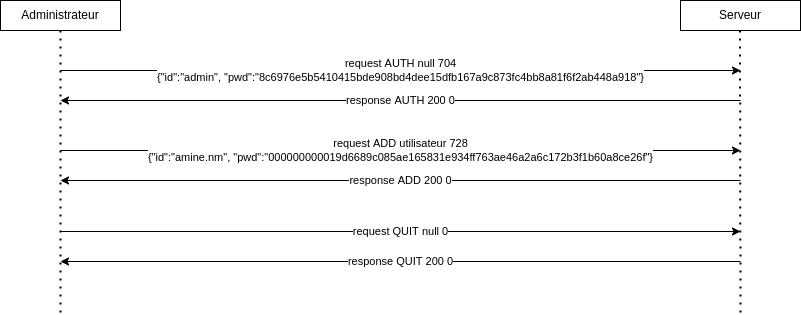
\includegraphics[width=\textwidth]{img/admin.png}
        \caption{Exemple sans erreur d'échanges entre l'administrateur et le serveur pour une création d'utilisateur}
    \end{figure}
    
    \begin{figure}[h]
        \centering
        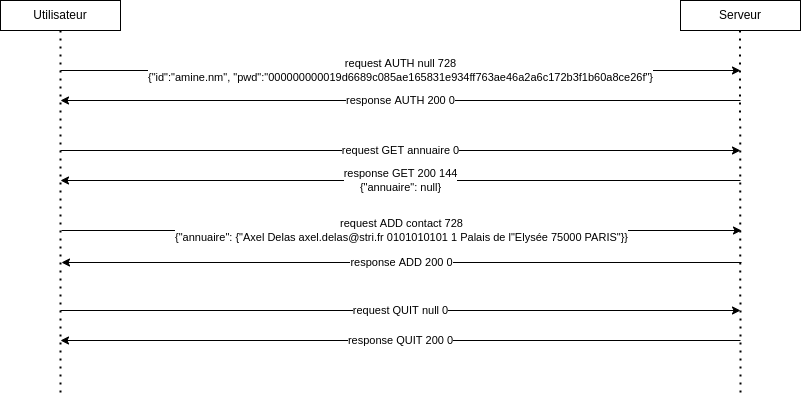
\includegraphics[width=\textwidth]{img/user.png}
        \caption{Exemple sans erreur d'échanges entre l'utilisateur et le serveur pour ajouter un contact dans l'annuaire}
    \end{figure}
    
    \begin{figure}[h]
        \centering
        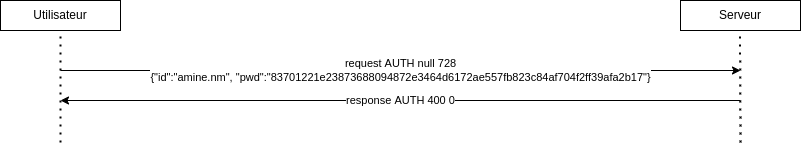
\includegraphics[width=\textwidth]{img/error.png}
        \caption{Exemple d'authentification avec de mauvais identifiants}
    \end{figure}
}

\clearpage

\section{Glossaire}
{
    \printglossary[title={}]
}
\end{document}
